% % % header removed
%\section{Experimentation and Data-set Description}


\subsection{Dataset and Study Area}

Two multi-frequency polarimetric SAR datasets from the AIRSAR system are used in this study. A C-, L-, P-band dataset  acquired over and agricultural area in Flevoland, Netherlands on 3 July 1991, and a C-, L-band dataset acquired over a forested area in Landes, France on 20 June 1991.
These 16-look datasets have a slant range resolution of \SI{6.66}{m} and an azimuth resolution of \SI{8.20}{m}. 
The Flevoland site consists of an agricultural area with large uniform fields with an average area of \SI{\sim20}{ha}. Extensive ground truth information from the campaign is available in literature~\cite{vissers1992groundtruth}.  
A $750\times700$ pixel subset is used to present the results in this paper. The crops present in this subset are Peas, Wheat, Rapeseed (R.Seed), Lucerne, Barley, Potato and Beet. Most of the crops are in the middle of their growth stage.  
The Landes site is a pine forest, with tree-patches of differing ages. A reference map is constructed from observation of polarimetric signatures.




%http://ieeexplore.ieee.org/document/5418883/#full-text-section
%\textcolor{red}{The Flevoland test site is a flat polder area with large uniform fields, with an average size (in 1991) of approximately 20 ha. For the 1991 growing season, a ground truth data set of 400 agricultural fields is available [26]. Though a multitemporal C-, L-, and P-band data set was collected during the MAC Europe campaign, only C- and L-band data of July 3, 1991, have been used. At this date, in the middle of the growing season, the main crops are characterized as follows: sugar beet fields have a cover of 40\%–60\% and a height of 20–35 cm; potato fields have a cover of 90\%–95\% and a height of 50–60 cm; wheat fields have a cover of 85\%–95\% and a height of 85–95 cm. The volumetric soil moisture level varies between 20\%–30\%. For the analysis presented in this paper a 640 × 640-pixel sub-image with a 46.8°–59.6° incidence angle range is used, for which 182 fields are available (Table II). The 16-look radar data have a slant range pixel spacing of 6.66 m in range and around 8.20 m in azimuth with an effective number of looks of approximately 14 per pixel for all bands. Spatial correlation decreases this number by approximately 30\% for C- and L-band. }


\subsection{Experimental Set-Up}

The ANN consists of two stages, an AE and a FF network. The AE consists of 5 hidden layers: 2 encode, 2 decode and 1 representational layer. The FF consists of 3 feed forward fully connected layers. First, the AE is trained in an unsupervised manner under the constraint of minimization of cross-entropy error between input $\bm{x_i}$ and output $\bm{x_i'}$ with the FF disconnected (see Figure~\ref{fig:ANN}). The learning rate is $l_r = 10^{-4}$ with a reduction by a factor of $\Gamma=0.1$ at every 2 training epochs. Optimization is performed using the ADAM solver with a momentum $\mu=0.95$ and weight decay $\beta=0.005$. The total labeled data is divided into 3 parts: training, test and validation which are selected at random. The proportions are 10\%, 30\% and 60\% of the total labeled data respectively. The training is balanced by selecting a fixed number of pixels per class randomly from the 10\% training pool.
The accuracy statistics are reported as an average of 5 runs on the validation set.  

After the training stage of the AE is complete, the representational layer is extracted and given as input to the FF network. The FF network is trained in a supervised manner with $l_r = 10^{-5}$, $\mu=0.92$ and $\beta=0.005$. The classification is obtained as output from the terminal layer of the FF network. 
%Single band, dual, clp and c+l+p

For comparison, the individual bands ($C$, $L$ and $P$), tensorized band pairs ($CL$, $CP$, $LP$),  tensorized triplet ($CLP$) and a simple band augmentation ($CLP_{+}$) are considered. For the individual bands, the input vector $\bm{x}$ is of dimension $1\times3$, while for tensorized pairs and triplets,  $\bm{x}$ is of dimension $1\times9$ and $1\times27$ respectively. 
%This forms a tensorized increased dimensional dataset.
% which require increased computation. To compare the benefit of using this high dimensional dataset,
The benefit of using the tensorization framework is demonstrated by comparing it  against the simple augmentation of all frequency bands. In the augmented case, the $1\times9$ resultant input vector is formed by appending individual frequency input vectors. The proposed framework is also compared with standard classification techniques like Support Vector Machine with a Radial Basis Function kernel (SVM-RBF) and Extreme Learning Machine
%~\cite{huang2006extreme} 
(ELM) network. The parameters used for comparison are automatically determined by standard techniques. 
For the SVM, $\gamma=0.125$ and $C=2^{-4}$. In the ELM, $N=1200$ with a sigmoid activation function is chosen.
%%>>>>>>>>>>>> TODO: Add a response 

It may be noted, that even though the Kronecker product operation is non-commutative, the operand ordering has no significant effect on the proposed algorithm since the AE is insensitive to the sequence of elements in the input vector. 
%The step size is 5 epochs, with a bath size of 
%5 AE layers
%3 FF network layers
%lr = 1E-5
%learning rate
% % % % % % % % % 
%number of nodes
% % % % % % % % %
%number of layers
%Data divided into training test and validation
%Advantage of a kronnecker reprentation - sparse etc.
%# post training
%After the training stage fo the AE is complete, the representational layer is abstracted.
%confidence measurement 
%how is the confidence measured
The null label node in the output layer is used to estimate the classification performance while qualitatively improving the results. If the output activation level of the node corresponding to the null label exceeds that of the other nodes, the corresponding pixel is considered unclassified and is excluded from the final classification output. The average normalized activation  of the successfully classified pixels is used as an estimation of the classification confidence. 



%%
% THe null label is used to estimate the confidence in the classification. If the activation of the null is more than others, that pixel is classed as unclassified. of all the pixels sucessfully classified the average uncertainity is computed from the activation value. this is reported in the table. It gives a good estimate of the ease of classification / seperability.

%Even thought the operation is non commutative. But in the proposed method all the elements are taken into account. 


%The classification performance 
% if Comparison is done with simple augmentation


\subsection{Results and Discussion}
\begin{figure}[t]
\centering
    \begin{subfigure}[b]{0.24\textwidth}
        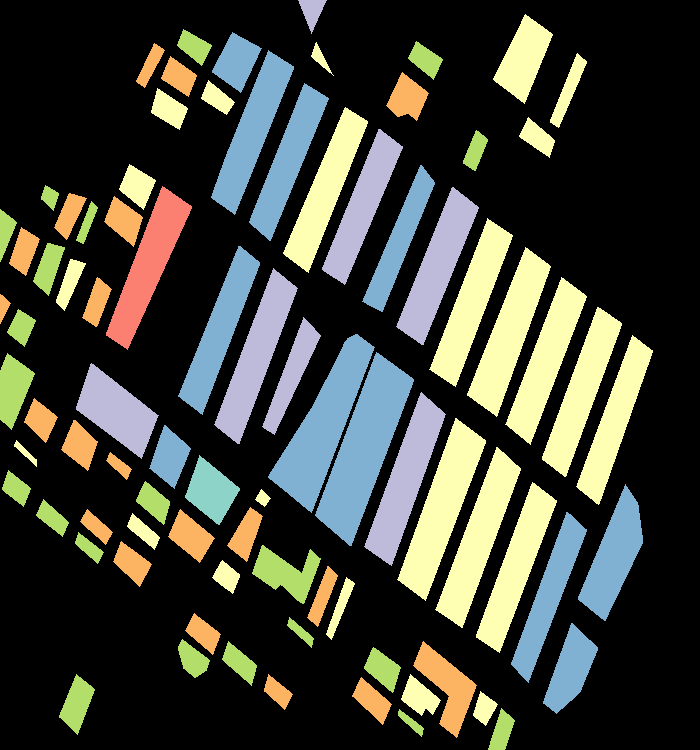
\includegraphics[width=\textwidth]{Figures/Kron/Validation_COLOUR}
        \caption{}
        \label{fig:Training}
    \end{subfigure}
     %~ %add desired spacing between images, e. g. ~, \quad, \qquad, \hfill etc. 
            %(or a blank line to force the subfigure onto a new line)
     \begin{subfigure}[b]{0.24\textwidth}
        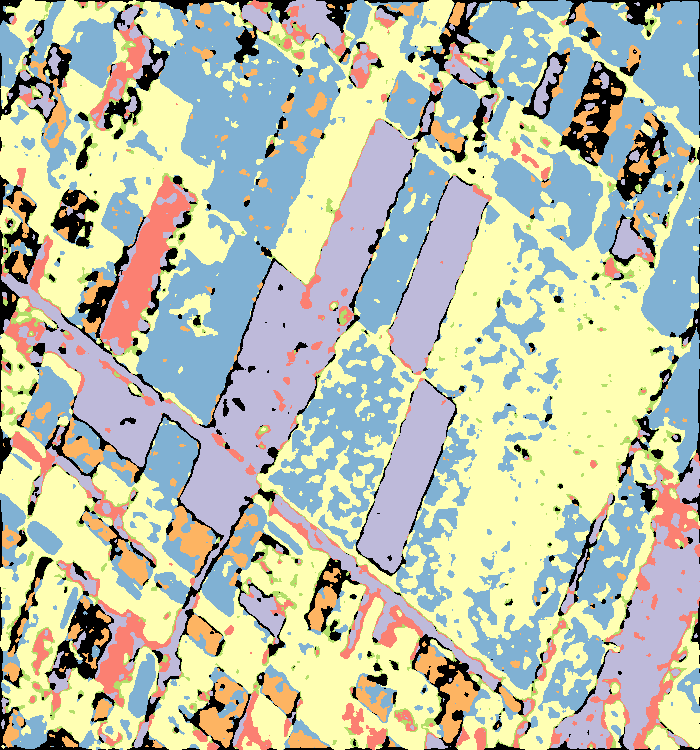
\includegraphics[width=\textwidth]{Figures/Kron/C_COLOUR}
        \caption{}
        \label{fig:C}
    \end{subfigure}
    %~ %add desired spacing between images, e. g. ~, \quad, \qquad, \hfill etc. 
      %(or a blank line to force the subfigure onto a new line)
    \begin{subfigure}[b]{0.24\textwidth}
        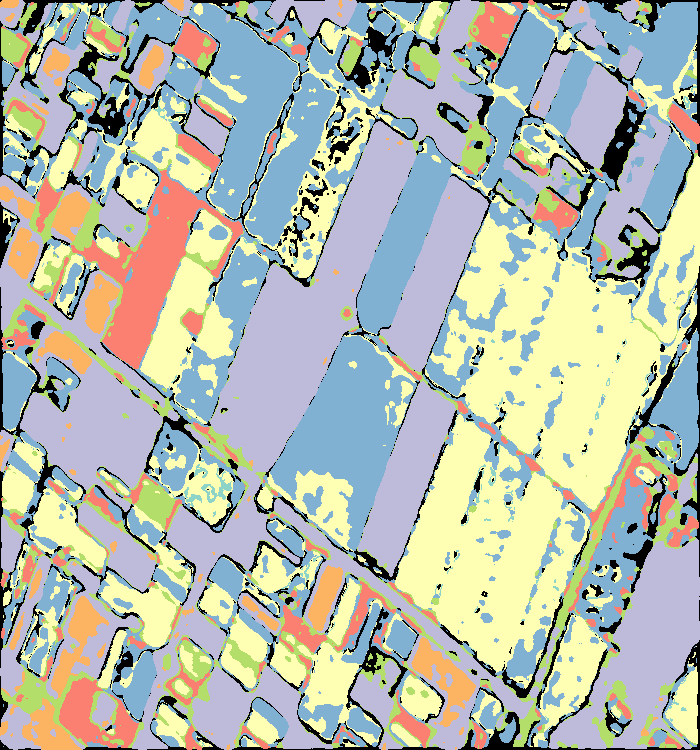
\includegraphics[width=\textwidth]{Figures/Kron/Ls_COLOUR}
        \caption{}
        \label{fig:L}
    \end{subfigure}
    %~ %add desired spacing between images, e. g. ~, \quad, \qquad, \hfill etc. 
    %(or a blank line to force the subfigure onto a new line)
    \begin{subfigure}[b]{0.24\textwidth}
        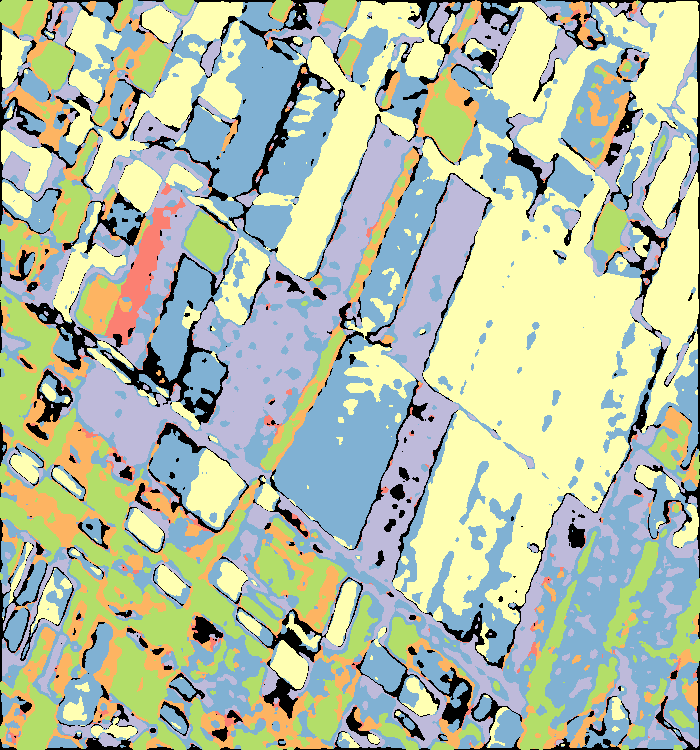
\includegraphics[width=\textwidth]{Figures/Kron/P_COLOUR}
        \caption{}
        \label{fig:P}
    \end{subfigure}
\begin{tabular}{llllllll}

\includegraphics[width=0.01\textwidth]{Figures/Kron/Legend/Pea} & Peas & 
\includegraphics[width=0.01\textwidth]{Figures/Kron/Legend/Wheat} & Wheat & 
\includegraphics[width=0.01\textwidth]{Figures/Kron/Legend/Rseed} & R.Seed & 
\includegraphics[width=0.01\textwidth]{Figures/Kron/Legend/Luc} & Lucerne  \\

\includegraphics[width=0.01\textwidth]{Figures/Kron/Legend/Barley} & Barley & 
\includegraphics[width=0.01\textwidth]{Figures/Kron/Legend/Potatoe} & Potato  & 
\includegraphics[width=0.01\textwidth]{Figures/Kron/Legend/Beet} & Beet &  & 
\end{tabular}
\caption{(a) Ground Truth.  Classification outputs of input vectors derived from individual (b) $C$ (c) $L$ (d) $P$ bands. }\label{fig:SingleBand}
\end{figure}



\begin{figure}[tbp]
\centering
        %~ %add desired spacing between images, e. g. ~, \quad, \qquad, \hfill etc. 
          %(or a blank line to force the subfigure onto a new line)
        \begin{subfigure}[b]{0.24\textwidth}
            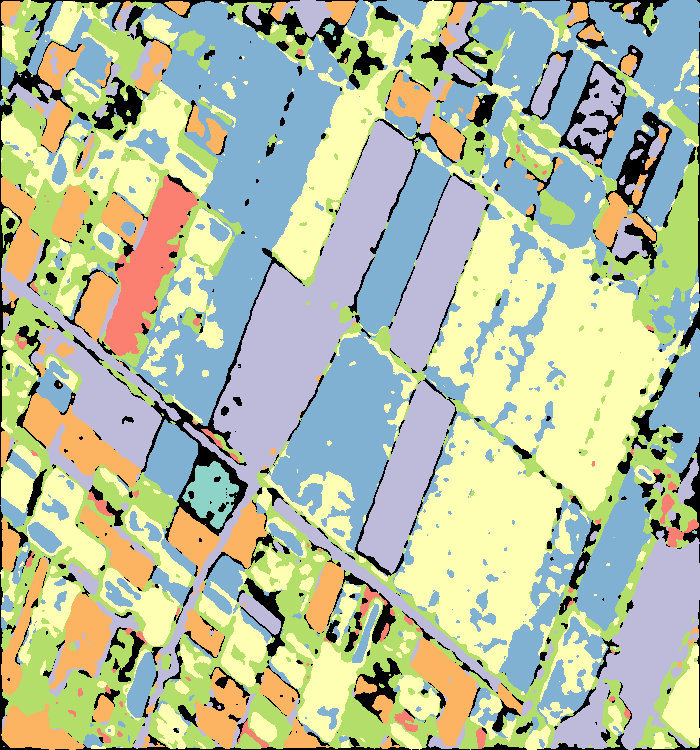
\includegraphics[width=\textwidth]{Figures/Kron/CL_COLOUR}
            \caption{}
            \label{fig:CL}
        \end{subfigure}
        ~ %add desired spacing between images, e. g. ~, \quad, \qquad, \hfill etc. 
        %(or a blank line to force the subfigure onto a new line)
        \begin{subfigure}[b]{0.24\textwidth}
            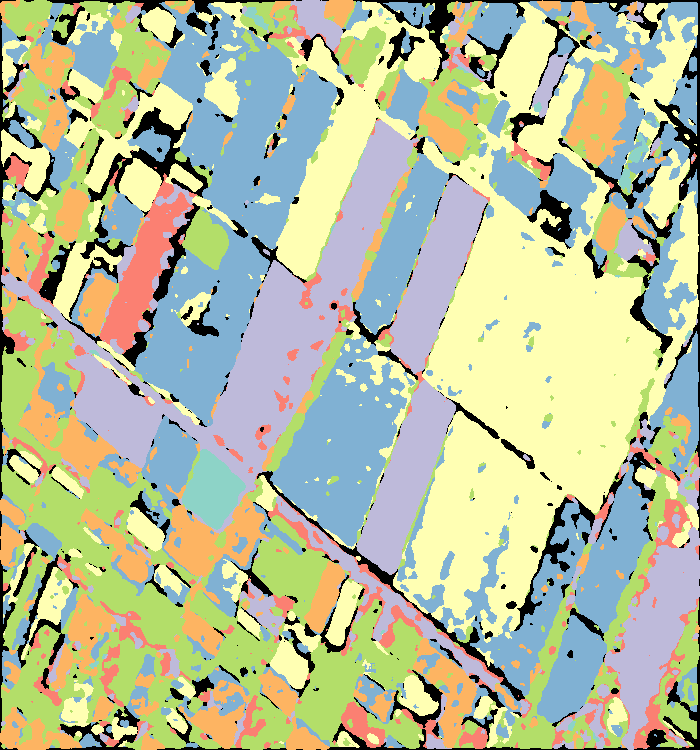
\includegraphics[width=\textwidth]{Figures/Kron/CP_COLOUR}
            \caption{}
            \label{fig:CP}
        \end{subfigure}
        ~ %add desired spacing between images, e. g. ~, \quad, \qquad, \hfill etc. 
          %(or a blank line to force the subfigure onto a new line)
        \begin{subfigure}[b]{0.24\textwidth}
            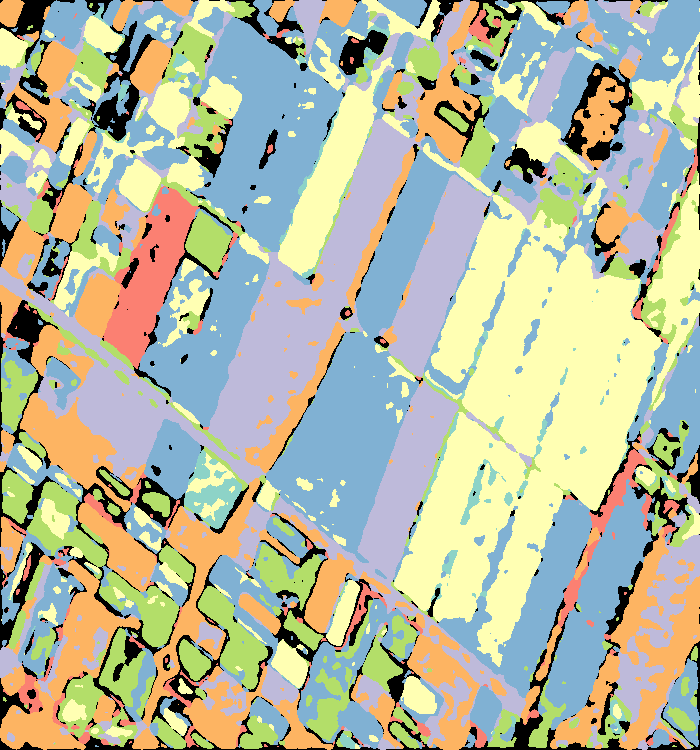
\includegraphics[width=\textwidth]{Figures/Kron/LP_COLOUR}
            \caption{}
            \label{fig:LP}
        \end{subfigure}
            ~ %add desired spacing between images, e. g. ~, \quad, \qquad, \hfill etc. 
            %(or a blank line to force the subfigure onto a new line)
            \begin{subfigure}[b]{0.24\textwidth}
                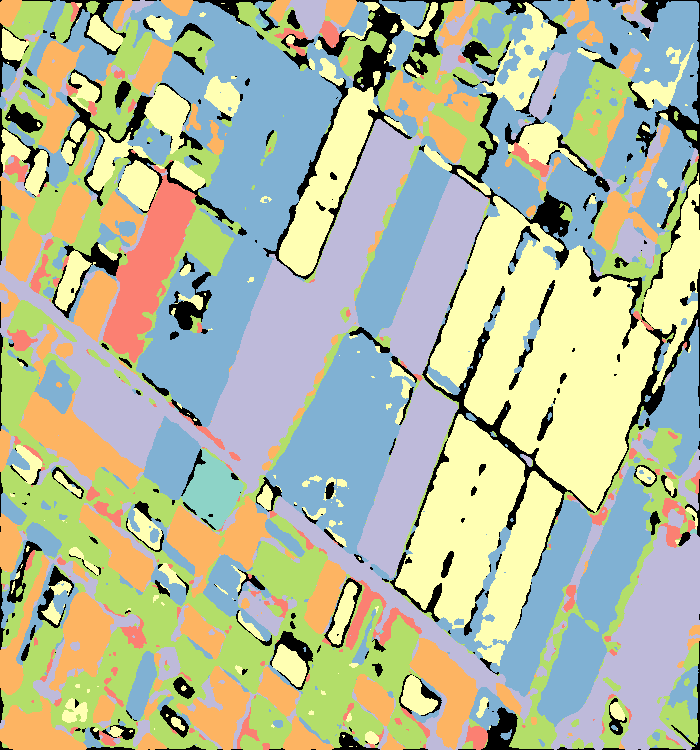
\includegraphics[width=\textwidth]{Figures/Kron/CLP_COLOUR}
                \caption{}
                \label{fig:CLP}
            \end{subfigure}
        ~
        \begin{subfigure}[b]{0.24\textwidth}
            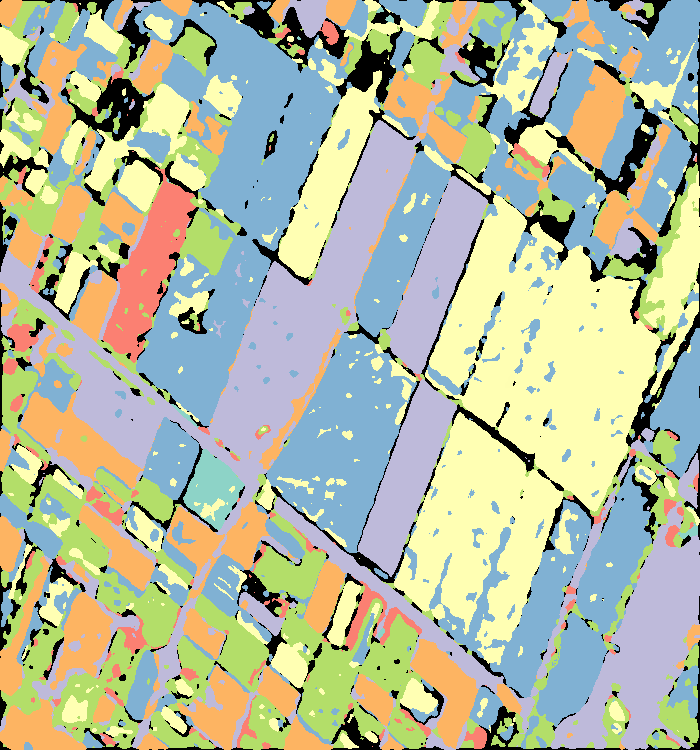
\includegraphics[width=\textwidth]{Figures/Kron/CLP2_COLOUR}
            \caption{}
            \label{fig:CLPaug}
        \end{subfigure}
        ~
        \begin{subfigure}[b]{0.24\textwidth}
                  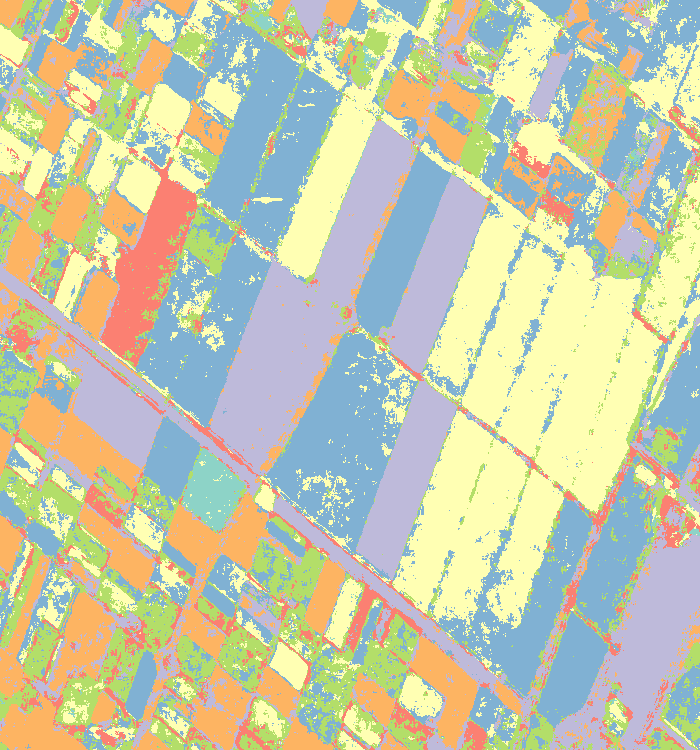
\includegraphics[width=\textwidth]{Figures/Kron/SVM_COLOUR}
                  \caption{}
                  \label{fig:SVM}
        \end{subfigure}
        ~
        \begin{subfigure}[b]{0.24\textwidth}
                        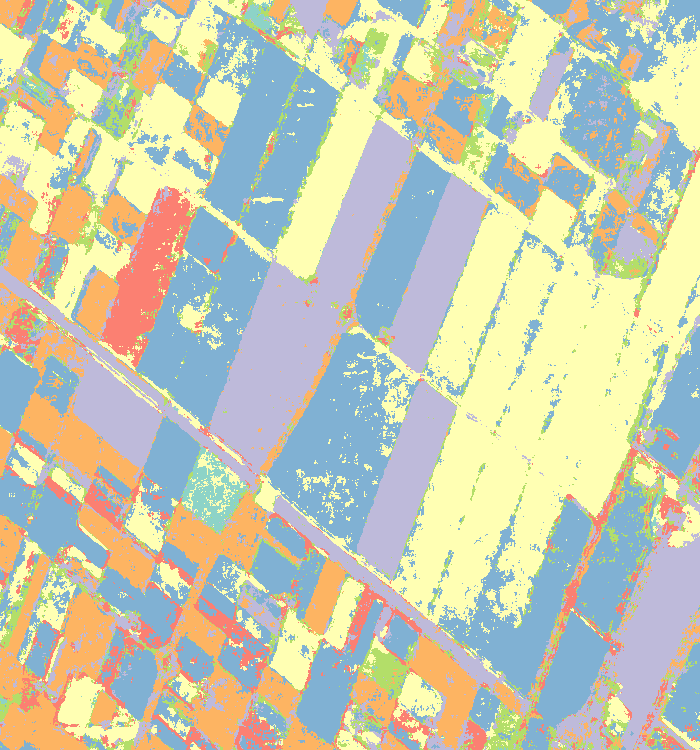
\includegraphics[width=\textwidth]{Figures/Kron/ELM_COLOR}
                        \caption{}
                        \label{fig:ELM}
        \end{subfigure}
%        \begin{tabular}{llllllllllllll}
%        
\includegraphics[width=0.01\textwidth]{Figures/Legend/Pea} & Peas & 
\includegraphics[width=0.01\textwidth]{Figures/Legend/Wheat} & Wheat & 
\includegraphics[width=0.01\textwidth]{Figures/Legend/Rseed} & R.Seed & 
\includegraphics[width=0.01\textwidth]{Figures/Legend/Luc} & Lucerne  &
%        
\includegraphics[width=0.01\textwidth]{Figures/Legend/Barley} & Barley & 
\includegraphics[width=0.01\textwidth]{Figures/Legend/Potatoe} & Potato  & 
\includegraphics[width=0.01\textwidth]{Figures/Legend/Beet} & Beet   
%        \end{tabular}
    \caption{Classification outputs of input vectors derived from (a) $CL$ (b) $CP$ (c) $LP$ (d) $CPL$ (e) $CLP_{+}$ band combinations with the proposed method and using (f) SVM-RBF (g) ELM methods. The SVM-RBF and ELM methods do not inherently generate a confidence map and are presented unmasked.}\label{fig:MultiFreq}
\end{figure}

%\begin{figure}[t]
%\centering
%                \includegraphics[width=0.2\textwidth]{Figures/Conf/CLP}
%   
%                
\includegraphics[width=0.1\textwidth]{Figures/Conf/grad}
%                \caption{CLP} 
%                \label{fig:CLPconf}
%\end{figure}

%\begin{figure*}[t]
%\centering
%        %~ %add desired spacing between images, e. g. ~, \quad, \qquad, \hfill etc. 
%          %(or a blank line to force the subfigure onto a new line)
%        \begin{subfigure}[b]{0.12\textwidth}
%            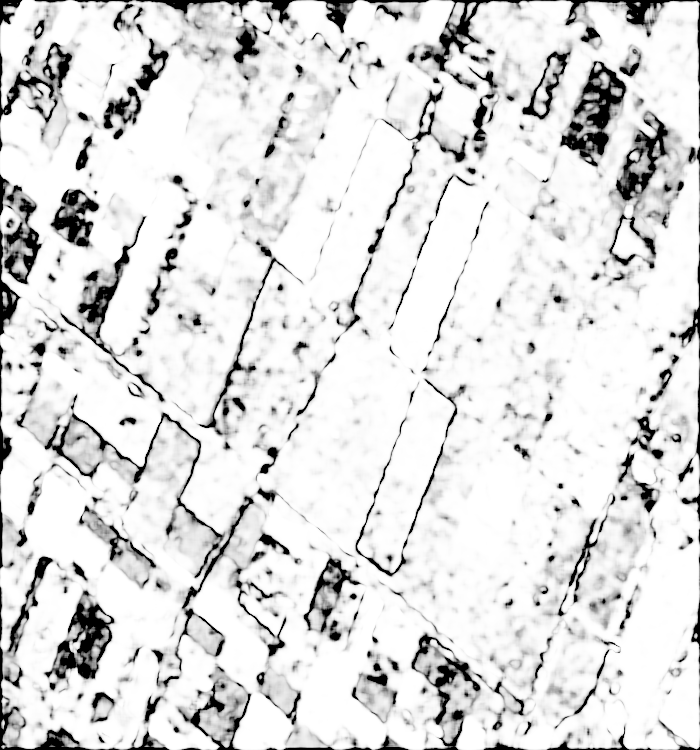
\includegraphics[width=\textwidth]{Figures/Conf/C}
%            \caption{C}
%            \label{fig:Cconf}
%        \end{subfigure}
%        ~ %add desired spacing between images, e. g. ~, \quad, \qquad, \hfill etc. 
%        %(or a blank line to force the subfigure onto a new line)
%        \begin{subfigure}[b]{0.12\textwidth}
%            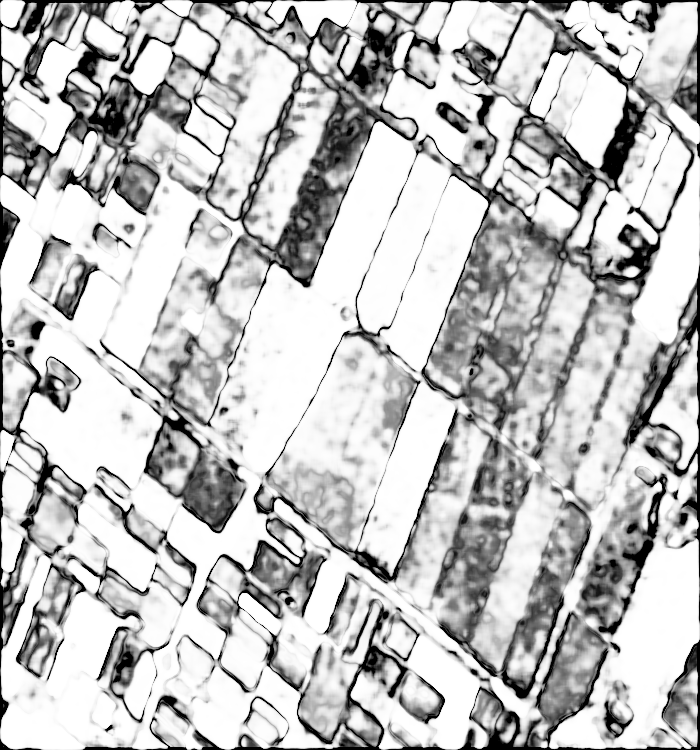
\includegraphics[width=\textwidth]{Figures/Conf/L}
%            \caption{L}
%            \label{fig:Lconf}
%        \end{subfigure}
%        ~ %add desired spacing between images, e. g. ~, \quad, \qquad, \hfill etc. 
%          %(or a blank line to force the subfigure onto a new line)
%        \begin{subfigure}[b]{0.12\textwidth}
%            \includegraphics[width=\textwidth]{Figures/Conf/P}
%            \caption{P}
%            \label{fig:Pconf}
%        \end{subfigure}
%        ~
%         \begin{subfigure}[b]{0.12\textwidth}
%                    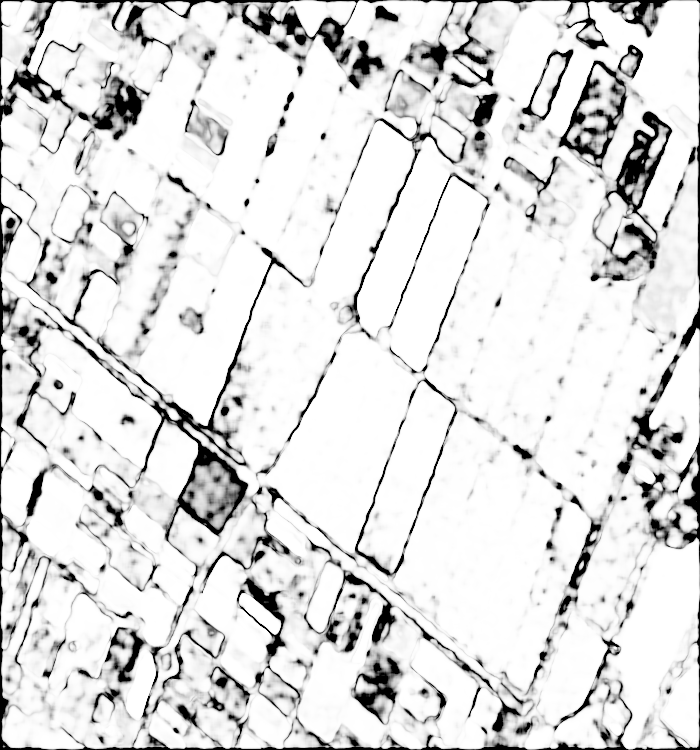
\includegraphics[width=\textwidth]{Figures/Conf/CL}
%                    \caption{CL}
%                    \label{fig:CLconf}
%                \end{subfigure}
%                ~ %add desired spacing between images, e. g. ~, \quad, \qquad, \hfill etc. 
%                %(or a blank line to force the subfigure onto a new line)
%                \begin{subfigure}[b]{0.12\textwidth}
%                    \includegraphics[width=\textwidth]{Figures/Conf/LP}
%                    \caption{LP}
%                    \label{fig:LPconf}
%                \end{subfigure}
%                ~ %add desired spacing between images, e. g. ~, \quad, \qquad, \hfill etc. 
%                  %(or a blank line to force the subfigure onto a new line)
%                \begin{subfigure}[b]{0.12\textwidth}
%                    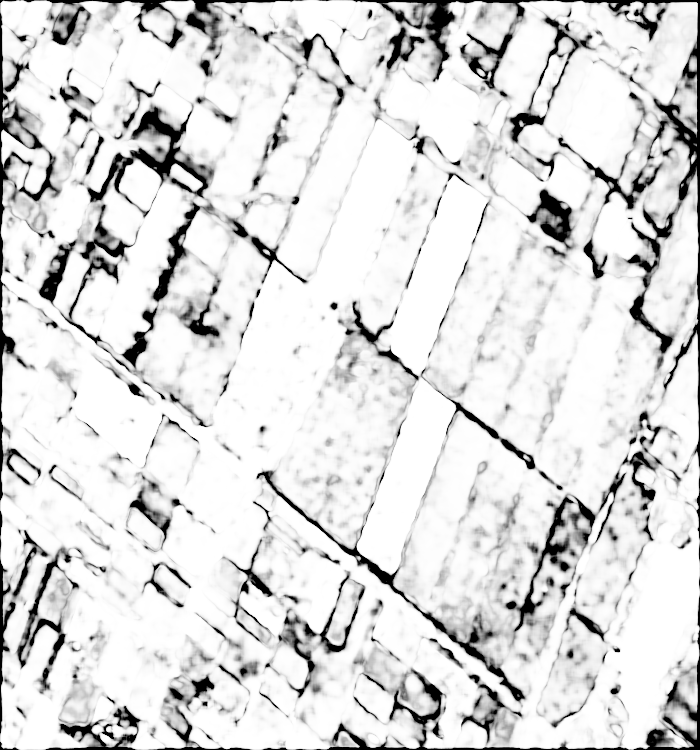
\includegraphics[width=\textwidth]{Figures/Conf/CP}
%                    \caption{CP}
%                    \label{fig:CPconf}
%                \end{subfigure}
%            ~ %add desired spacing between images, e. g. ~, \quad, \qquad, \hfill etc. 
%            %(or a blank line to force the subfigure onto a new line)
%            \begin{subfigure}[b]{0.12\textwidth}
%                \includegraphics[width=\textwidth]{Figures/Conf/CLP}
%                \caption{CLP}
%                \label{fig:CLPconf}
%            \end{subfigure}
%            
\includegraphics[width=0.1\textwidth]{Figures/Conf/grad}
%    \caption{MultiBand}\label{fig:Conf}
%\end{figure*}


%\begin{figure}[t]
%\centering
%        %~ %add desired spacing between images, e. g. ~, \quad, \qquad, \hfill etc. 
%          %(or a blank line to force the subfigure onto a new line)
%        \begin{subfigure}[b]{0.12\textwidth}
%            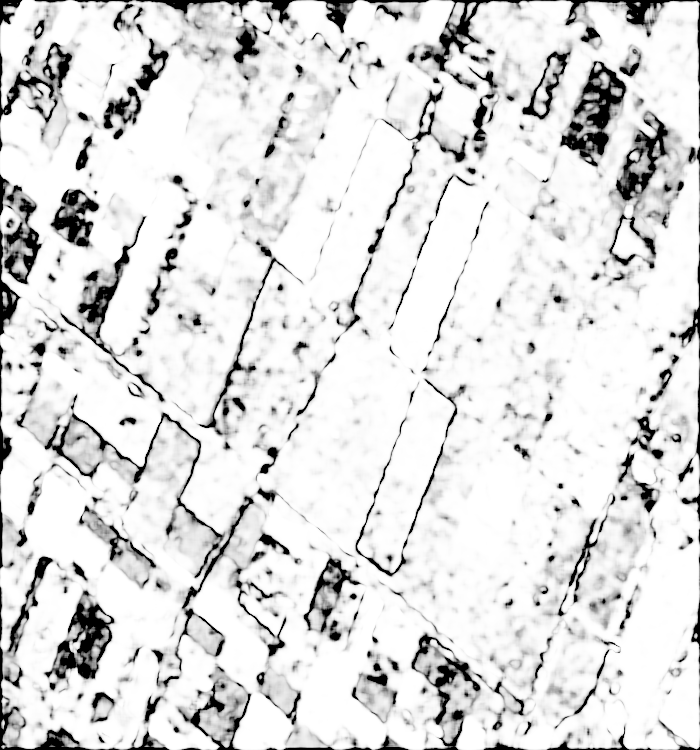
\includegraphics[width=\textwidth]{Figures/Conf/C}
%            \caption{C}
%            \label{fig:Cconf}
%        \end{subfigure}
%        ~ %add desired spacing between images, e. g. ~, \quad, \qquad, \hfill etc. 
%        %(or a blank line to force the subfigure onto a new line)
%        \begin{subfigure}[b]{0.12\textwidth}
%            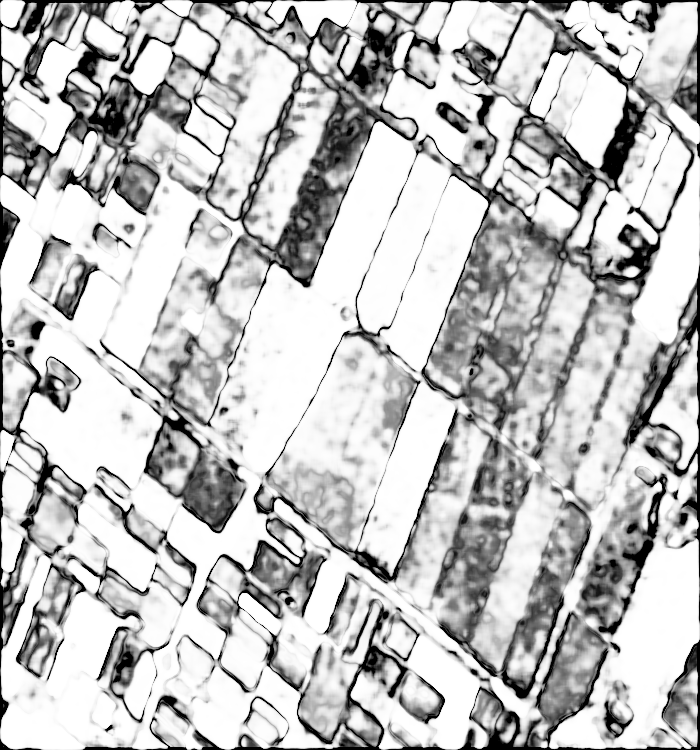
\includegraphics[width=\textwidth]{Figures/Conf/L}
%            \caption{L}
%            \label{fig:Lconf}
%        \end{subfigure}
%        ~ %add desired spacing between images, e. g. ~, \quad, \qquad, \hfill etc. 
%          %(or a blank line to force the subfigure onto a new line)
%        \begin{subfigure}[b]{0.12\textwidth}
%            \includegraphics[width=\textwidth]{Figures/Conf/P}
%            \caption{P}
%            \label{fig:Pconf}
%        \end{subfigure}
%        ~
%         \begin{subfigure}[b]{0.12\textwidth}
%                    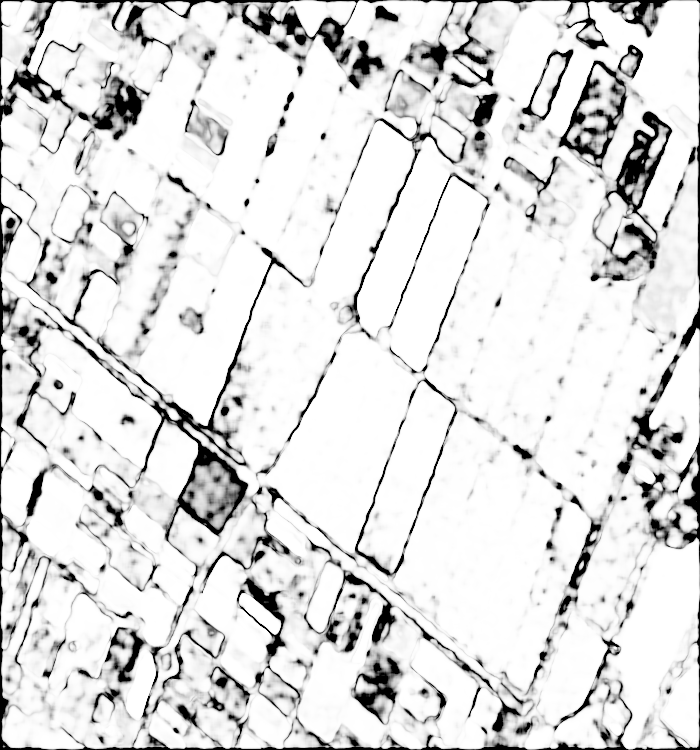
\includegraphics[width=\textwidth]{Figures/Conf/CL}
%                    \caption{CL}
%                    \label{fig:CLconf}
%                \end{subfigure}
%                ~ %add desired spacing between images, e. g. ~, \quad, \qquad, \hfill etc. 
%                %(or a blank line to force the subfigure onto a new line)
%                \begin{subfigure}[b]{0.12\textwidth}
%                    \includegraphics[width=\textwidth]{Figures/Conf/LP}
%                    \caption{LP}
%                    \label{fig:LPconf}
%                \end{subfigure}
%                ~ %add desired spacing between images, e. g. ~, \quad, \qquad, \hfill etc. 
%                  %(or a blank line to force the subfigure onto a new line)
%                \begin{subfigure}[b]{0.12\textwidth}
%                    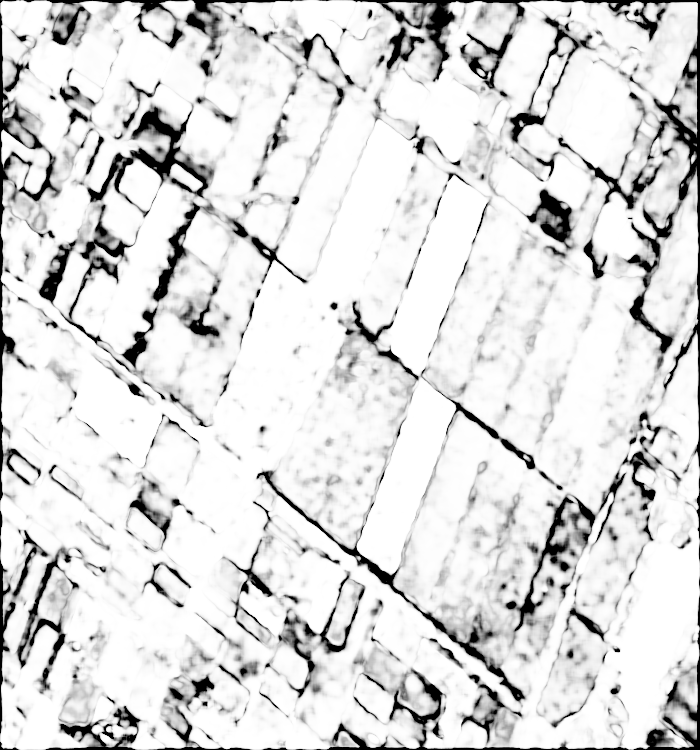
\includegraphics[width=\textwidth]{Figures/Conf/CP}
%                    \caption{CP}
%                    \label{fig:CPconf}
%                \end{subfigure}
%            ~ %add desired spacing between images, e. g. ~, \quad, \qquad, \hfill etc. 
%            %(or a blank line to force the subfigure onto a new line)
%            \begin{subfigure}[b]{0.12\textwidth}
%                \includegraphics[width=\textwidth]{Figures/Conf/CLP}
%                \caption{CLP}
%                \label{fig:CLPconf}
%            \end{subfigure}
%            
%            
\includegraphics[width=0.1\textwidth]{Figures/Conf/grad}
%    \caption{MultiBand}\label{fig:Conf}
%\end{figure}

%%%%%%%%%%%%%%%%%%%%%%%%%%%%%%%%%%%%%%%%%%%%%%
%Confidence MAPS %% Removed for space
%%%%%%%%%%%%%%%%%%%%%%%%%%%%%%%%%%%%%%%%%%%%%%
\begin{figure}[tbp]
\centering
        %~ %add desired spacing between images, e. g. ~, \quad, \qquad, \hfill etc. 
          %(or a blank line to force the subfigure onto a new line)
        \begin{subfigure}[b]{0.3\textwidth}
            \includegraphics[width=\textwidth]{Figures/Kron/Conf/P}
            \caption{}
            \label{fig:Pconf}
        \end{subfigure}
        ~
        \begin{subfigure}[b]{0.3\textwidth}
            \includegraphics[width=\textwidth]{Figures/Kron/Conf/LP}
            \caption{}
            \label{fig:CPconf}
        \end{subfigure}
            ~ %add desired spacing between images, e. g. ~, \quad, \qquad, \hfill etc. 
            %(or a blank line to force the subfigure onto a new line)
            \begin{subfigure}[b]{0.3\textwidth}
                \includegraphics[width=\textwidth]{Figures/Kron/Conf/CLP}
                \caption{}
                \label{fig:CLPconf}
            \end{subfigure}
          
            
\includegraphics[width=0.1\textwidth]{Figures/Kron/Conf/grad}
    \caption{Confidence maps generated from the classification using (a) $P$ (b) $CL$ (c) $CLP$ band combinations.}\label{fig:Conf}
\end{figure}
%%%%%%%%%%%%%%%%%%%%%%%%%%%%%%%%%%%%%%%%%%%%%%

%%%%%%%%%%%%%%%%%%
% Tables

\begin{table}[tbp]
	\centering
	\caption{Class Wise Overall Accuracy}
	\label{tab:class}
	\begin{tabularx}{\columnwidth}{XXXXXXXXX}
		\hline \noalign{\vskip 0.5mm} 
		$\diagup$ & $C$    & $L$    & $P$    & $CL$   & $LP$   & $CP$   & $CLP$ & $CLP_+$  \\ \hline \noalign{\vskip 0.3mm}
		Peas     & 0.40 & 0.26 & 0.00 & 0.84 & 0.66 & 0.99 & \textbf{1.00} & 0.86\\
		Wheat    & 0.70 & 0.81 & 0.91 & 0.84 & 0.89 & \textbf{0.95} & 0.93 & 0.90\\
		R.Seed & 0.81 & 0.97 & 0.88 & 0.99 & 0.99 & 0.99 & \textbf{1.00} & 0.98\\
		Lucerne  & 0.82 & 0.94 & 0.07 & 0.98 & 0.91 & 0.85 & \textbf{0.99} & 0.97\\
		Barley   & 0.73 & 0.77 & 0.76 & 0.89 & 0.97 & 0.93 & \textbf{0.98} & 0.95\\
		Potato   & 0.71 & 0.31 & 0.31 & 0.89 & 0.69 & 0.70 & \textbf{0.92} & 0.90\\
		Beet     & 0.32 & 0.27 & 0.32 & 0.56 & 0.68 & 0.63 & \textbf{0.90} & 0.75\\ \hline  \noalign{\vskip 1mm} 
		%         &        &       &          & \vline    &        &        &         \\
		% Overall  & Acc.   & 98.22\% &        &       &        &Kappa   & 0.94   \\ \hline
	\end{tabularx}
\end{table}

\begin{table}[tbp]
	\caption {Table of Accuracy, Kappa and Confidence.}
	\label{tab:OAnACC}
	\centering
	\begin{tabular}{l c c c}
		\hline \noalign{\vskip 0.5mm} 
		Band(s) & Accuracy ($\%$) & Kappa & Confidence \\ \hline \noalign{\vskip 1mm} 
		$C$ & 89.78 & 0.62 & 0.86\\
		$L$ & 90.86 & 0.64 & 0.80\\ 
		$P$ & 90.75 & 0.65 & 0.87\\ 
		$CL$ & 95.58 &  0.84 & 0.92\\ 
		$LP$ & 89.79 & 0.62 & 0.92\\ 
		$CP$ & 96.59 & 0.88 & 0.91\\
		${CLP}$ (Proposed) & {98.23} & {0.94} & {0.93}\\ 
		$CLP_{+}$ & 95.23 & 0.89 & 0.92\\ \hline  \noalign{\vskip 1mm} 
		$SVM-RBF$ & 96.48 & 0.89 & --- \\ 
		$ELM$ & 95.70 & 0.82 & --- \\ \hline
	\end{tabular}
\end{table}

%\begin{table}[!t]
%    \caption {Average confidence}
%    \label{tab:conf}
%    \centering
%    \begin{tabular}{l c c}
%        \hline \noalign{\vskip 0.5mm} 
%Band(s) & Confidence &  \\
%C       & 0.86       &  \\
%L       & 0.84       &  \\
%P       & 0.87       &  \\
%CL      & 0.92       &  \\
%LP      & 0.92       &  \\
%CP      & 0.91       &  \\
%CLP     & 0.93       &  \\ \hline  \noalign{\vskip 1mm} 
%        
%    \end{tabular}
%\end{table}



\begin{table}[tp]
	\centering
	\caption{Confusion Matrix for $CLP$}
	\label{tab:cmCLP}
	\begin{tabularx}{\columnwidth}{XXXXXXXX|X}
		\hline \noalign{\vskip 0.5mm} 
		$(\%)$   & Peas & Wheat      & R.Seed   & Lucerne      & Barley     & Potato   & Beet & Supp.     \\ \hline \noalign{\vskip 0.3mm} 
		Pees     & 100 & 0.00  & 0.00     & 0.00   & 0.00   & 0.00   & 0.00 & 2055 \\
		Wheat    & 0.00   & 93.90 & 0.04     & 0.03   & 5.96   & 0.00   & 0.07 & 56060 \\
		R.Seed   & 0.00   & 0.00  & 100   & 0.00   & 0.00   & 0.00   & 0.00 & 25994 \\
		Lucerne  & 0.00   & 0.00  & 0.00     & 99.88  & 0.00   & 0.00   & 0.12 & 4935 \\
		Barley   & 0.00   & 2.03  & 0.00     & 0.00   & 97.93  & 0.00   & 0.04 & 45497 \\
		Potato   & 0.00   & 0.00  & 0.78     & 0.00   & 7.15   & 91.97  & 0.10 & 17035 \\
		Beet     & 0.00   & 3.63  & 0.07     & 3.63   & 2.82   & 0.04   & 89.81 & 14974 \\ \hline  %\noalign{\vskip 1mm} 
		%         &        &       &          & \vline    &        &        &         \\
		Prec.  & 2055   & 54107 &   26160     &   5489    &  49537      &15673  & 13529 &  \\ %166550 \\ 
		Overall  & Acc.   & 98.23\% &        &       &        &$\kappa$   & 0.94 &  \\ \hline
	\end{tabularx}
\end{table}
%%%%%%%%%%%%%%%%%%%%%%%%%%%%%%%%%%%%%%%%%%%%%%%%%%%









\subsubsection{Flevoland Dataset}
%For the Flevoland dataset, 
The result of classification using individual frequency bands is shown in Figure~\ref{fig:SingleBand}. The L-band has the best classification accuracy amongst the three individual bands with an overall accuracy of $90.86\%$ and Cohen's kappa ($\kappa$) of $0.64$. This is followed by the P-band with $90.75\%$ and C-band with $89.79\%$. 
Classwise accuracies for each band or band-combinations are shown in Table~\ref{tab:class}. The values tabulated in bold indicate the best performance combination for the particular class. 
The longer wavelength of the P-band allows it a high penetration capability. This renders broad leaf, sparse crops like peas, potatoes and sugar beet nearly invisible to the radar leading to misclassification. Even at a comparatively shorter wavelength of L-band, the accuracy of classification of the pea crop is only $26.21\%$. 
At this frequency band, it is mostly confused with wheat. 
The best classification for this crop is obtained using C-band with a classification accuracy of $40.01\%$. 

Sugar-beet which has a height of \SI{24}-\SI{30}{cm} and has a cover of about $40\% - 60\%$ is also misclassified by all three bands. 
%At C-band and L-band it is primarily confused with wheat, while at P-band it is misclassified as barley. 
Potato crops are taller and have a height of \SI{50}-\SI{60}{cm} with a cover of $90\% - 95\%$. These are classified reasonably well with the C-band with an accuracy of 71.16\%, but poorly so with L- and P-band with accuracies of $30.80\%$ and $30.93\%$, respectively. 
Long stem vegetative crops like wheat, with a cover of $85\% - 95\%$ and a height of \SI{85}-\SI{95}{cm}, are well classified with all three frequencies. 
This disparity in performance is indicative of the differences in information content for each crop at different sensing wavelengths. This can be potentially exploited by combining information from different bands to improve the classification performance. 



%40\%–60\% and a height of 20–35 cm; potato fields have a cover of 90\%–95\% and a height of 50–60 cm; wheat fields have a cover of 85\%–95\% and a height of 85–95 cm



The result of multi-frequency classifications with the proposed approach is shown in Figure~\ref{fig:MultiFreq}. The combination of information from different bands is able to improve the classification accuracy. The overall accuracies for individual and combined frequency bands along with two standard methods are reported in Table~\ref{tab:OAnACC}. 
It can be seen that the tensor combination of all three bands is the most informative and has the best classification performance with an overall accuracy of $98.23\%$ with $\kappa = 0.94$. In this combination, all classes are correctly identified with the potatoes and sugar beet having the least accuracies at $91.97\%$ and $89.82\%$, respectively. These classes, however, have not been significantly confused with the others, rather they have remained unclassified due to low confidence. This may be due to broad leaves and the relative size of the crop.
%Further improvement in performance can be achieved in future by developing a network architecture which is able to improve this. 
%
%%%%%%%>>>>>>>>>>>>>V3+
The performance of the proposed algorithm is identical to the state-of-the art approach reported in~\cite{7375754}. However, the proposed method being non-parametric makes no \textit{a-priori} assumptions about the distribution of the data. 


Among the dual frequency combinations,  $CP$ has the highest performance with an overall classification accuracy of $96.59\%$ with $\kappa = 0.88$. This combination contains the most diverse information, with the $C$ band being sensitive to scattering from the vegetation canopy, while the $P$ band is able to penetrate into deeper layers of vegetation. This is followed by the $LP$ combination with an overall classification accuracy of $96.40\%$ with $\kappa = 0.87$. Finally, the $CL$ combination has the lowest performance, with an overall accuracy of $95.57\%$ with $\kappa = 0.84$. However, it outperforms classification using individual bands. 
The multilayer information content carried by each (C-, L-, P-) band allows for better crop classification by integrating multi-frequency information. 
It is also seen that tensorization ($CLP$) is able to outperform simple band augmentation ($CLP_{+}$), and also the SVM-RBF and ELM approaches. Since the confidence map generation was not a part of the SVM-RBF and ELM techniques, they are presented unmasked. However explicit generation of confidence maps might be possible with different strategies in each technique.
The confusion matrix for classification using $CLP$ combination by the proposed method is presented in Table~\ref{tab:cmCLP}. Wheat is the most significant class in the dataset and is classified with an accuracy of $93.91\%$, with the rest being confused with barley. Among the crops present, the beet crop is misclassified with most other crops.
%%%%%%%%%%%%v3
The confidence maps for the band combinations with the least classification uncertainty for single, double and triple band combinations are shown in Figure~\ref{fig:CLPconf}. In particular, for $CLP$ combination (Figure~\ref{fig:CLPconf}), the field boundaries are automatically masked out due to low confidence, thus improving the quality of the classification. 

%%%%%%%%%%%%%%%%%%% V3+

\subsubsection{Landes Dataset}
To establish the robustness of the results an experiment is conducted on the Landes dataset with two frequency bands. The classification results are presented in Figure~\ref{fig:secondSet}. 
The tensorized pair $CL$ has an overall accuracy of $96.23\%$ with $\kappa=0.94$. This exceeds the classification performance obtained by simple augmentation ($CL_+$), which has an overall accuracy of $92.15\%$ with $\kappa=0.91$. For individual bands, the L-band, with an overall accuracy of  $89.73\%$ with $\kappa=0.70$, outperforms the C-band alone, which has an overall accuracy of  $77.42\%$ with $\kappa=0.62$. In this case, the greater penetration ability of L-band is crucial in being able to segregate the age of the trees, since return from the top foliage of the tree is nearly identical irrespective of their ages. 
%secondSet

%%%%%%%%%%%%%%%%%%%%%%%%%%%%%%%%%%%%%V3+
\begin{figure}[t]
	\centering
	\begin{subfigure}[b]{0.23\textwidth}
		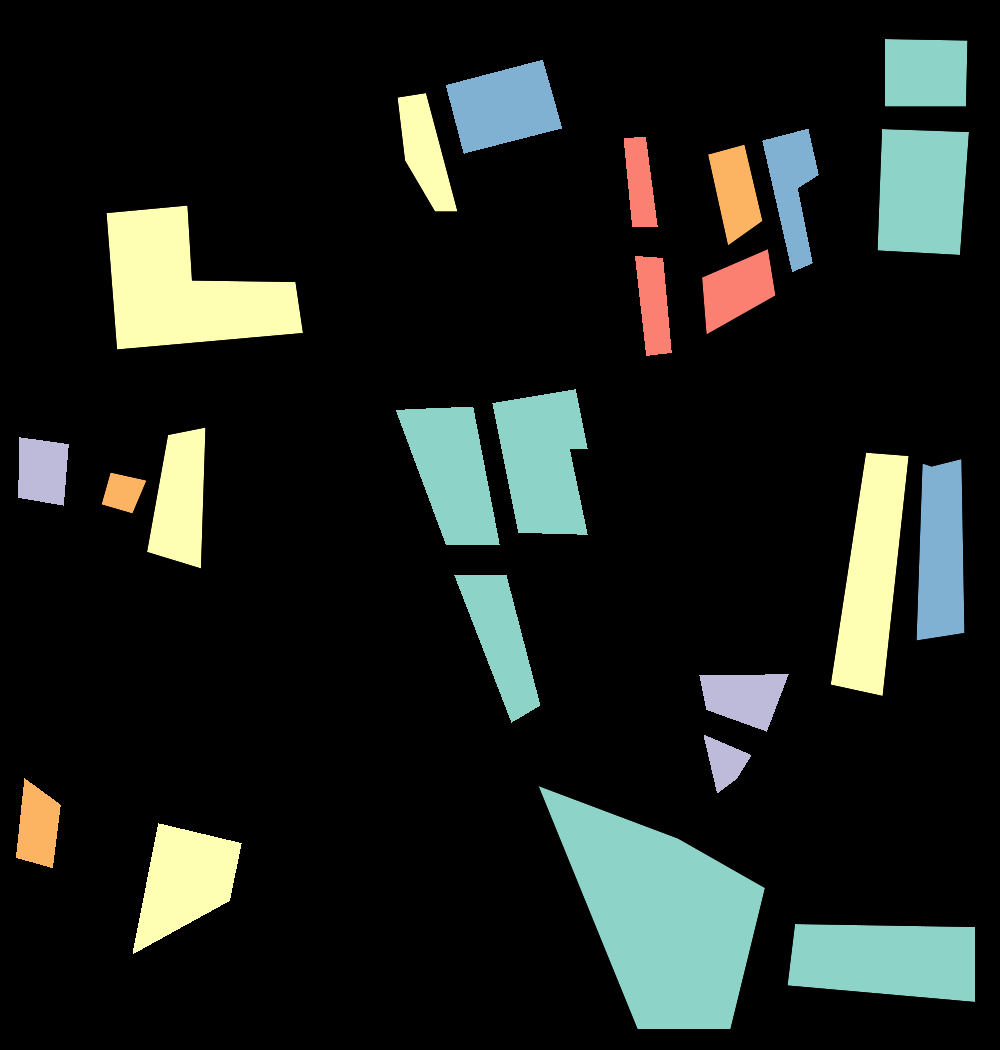
\includegraphics[width=\textwidth]{Figures/Kron/Review/GT}
		\caption{}
		\label{fig:Training}
	\end{subfigure}
	%~ %add desired spacing between images, e. g. ~, \quad, \qquad, \hfill etc. 
	%(or a blank line to force the subfigure onto a new line)
	\begin{subfigure}[b]{0.23\textwidth}
		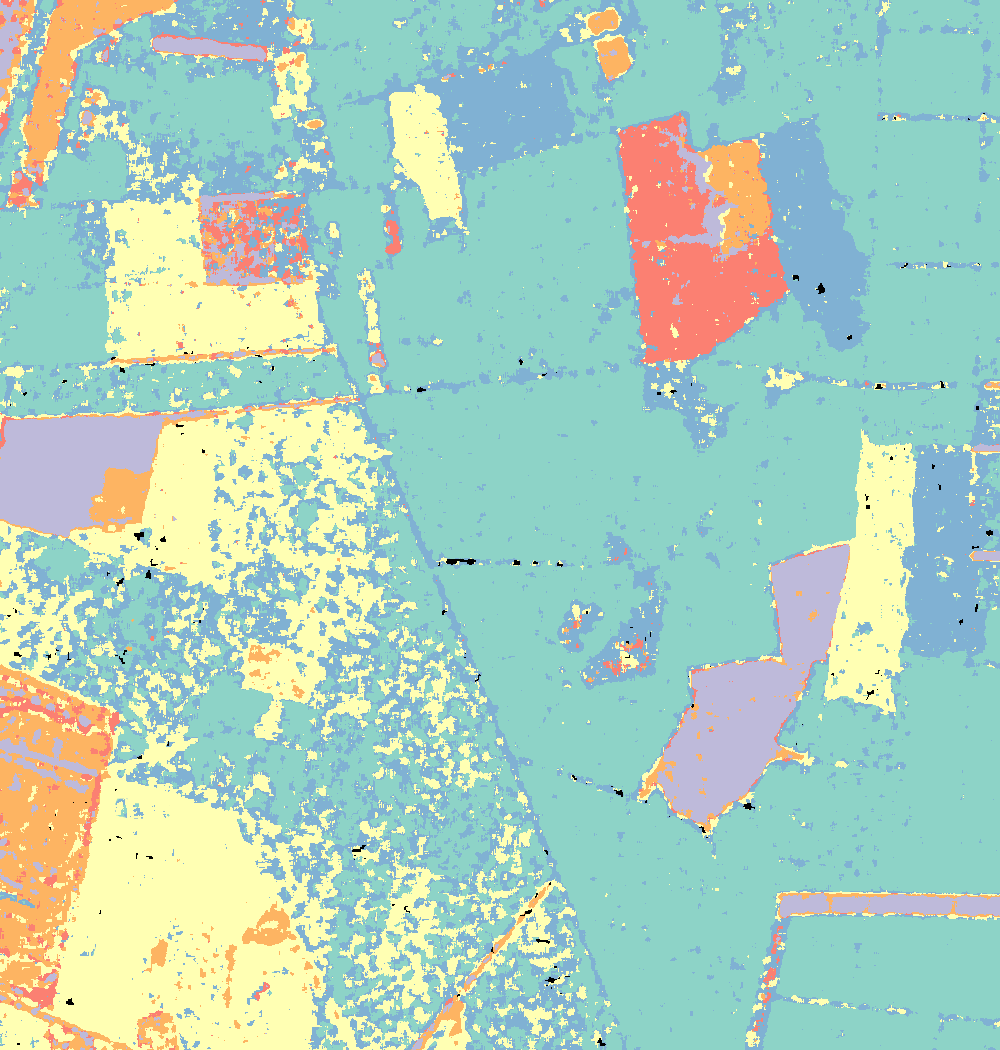
\includegraphics[width=\textwidth]{Figures/Kron/Review/CL_raw_COLOUR_PR_0_185_1000_1050_MASK}
		\caption{}
		\label{fig:C}
	\end{subfigure}
	%~ %add desired spacing between images, e. g. ~, \quad, \qquad, \hfill etc. 
	%(or a blank line to force the subfigure onto a new line)
	\begin{subfigure}[b]{0.23\textwidth}
		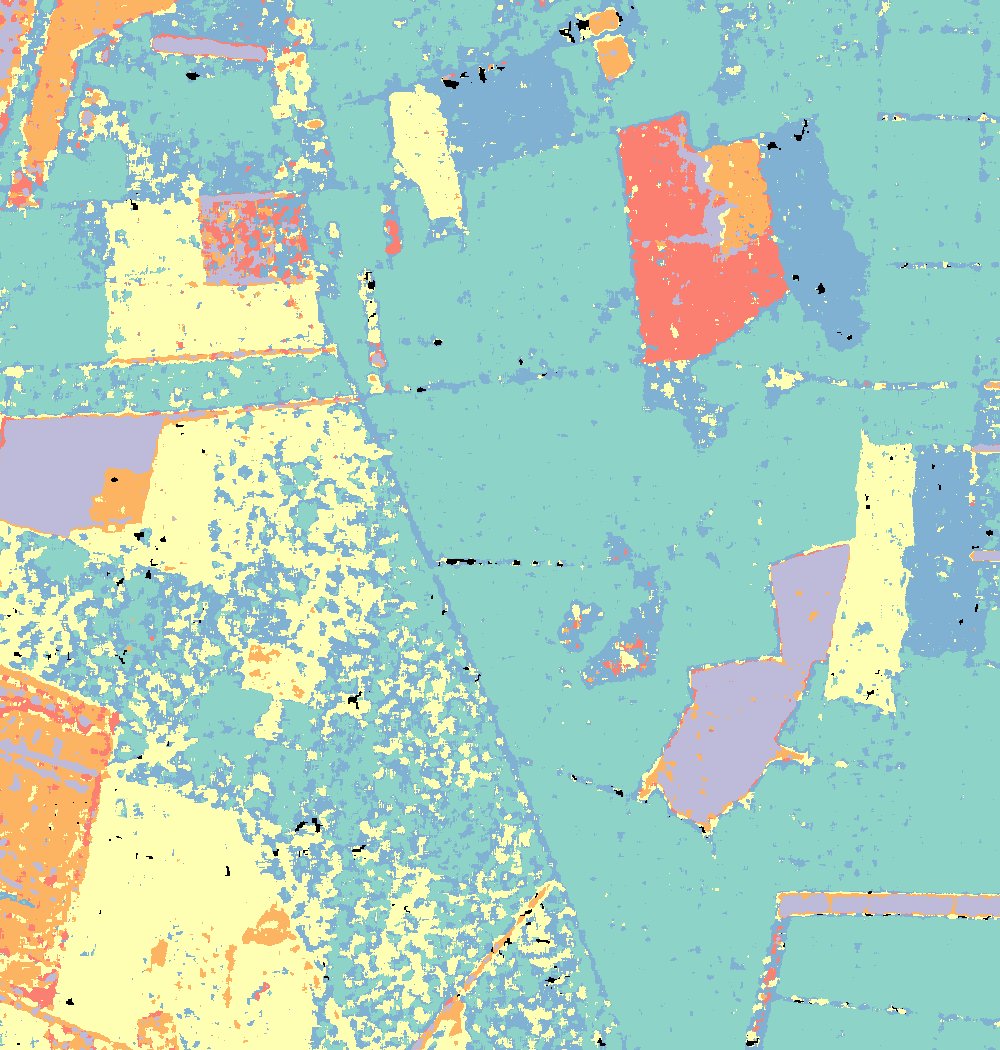
\includegraphics[width=\textwidth]{Figures/Kron/Review/C+L_RAW+COLOUR_CROP_MASK}
		\caption{}
		\label{fig:L}
	\end{subfigure}
	%~ %add desired spacing between images, e. g. ~, \quad, \qquad, \hfill etc. 
	%(or a blank line to force the subfigure onto a new line)
	\begin{subfigure}[b]{0.23\textwidth}
		\includegraphics[width=\textwidth]{Figures/Kron/Review/L_COLOUR_PR_CROP_MASK}
		\caption{}
		\label{fig:P}
	\end{subfigure}
	\begin{tabular}{lllllllllll}
		\includegraphics[width=0.01\textwidth]{Figures/Kron/Legend/Pea} & C1 & \includegraphics[width=0.01\textwidth]{Figures/Kron/Legend/Wheat} & C2 & \includegraphics[width=0.01\textwidth]{Figures/Kron/Legend/Rseed} & C3 & \includegraphics[width=0.01\textwidth]{Figures/Kron/Legend/Luc} & C4 &
		\includegraphics[width=0.01\textwidth]{Figures/Kron/Legend/Barley} & C5 &
		 %\includegraphics[width=0.01\textwidth]{Figures/Legend/Potatoe} & Potato  & %\includegraphics[width=0.01\textwidth]{Figures/Legend/Beet} & Beet &  & 
	\end{tabular}
	\caption{(a) Reference Image.  Classification outputs of input vectors derived from individual (b) $CL$ (c) $CL_+$ (d) $L$ bands. }\label{fig:secondSet}
\end{figure}
%%%%%%%%%%%%%%%%%%%%%%%%%%%%%%%%%%%%%%%%%%



%%%%%%%%%%%%%%%%%%%%%%%%%%%%%%%%%%%%%%%%5
%unclass no showm 
%Crops like peas which are misclassified in the 
%confidence of classification of beet is least
%Discsuss how aug has less dimension by performs less

%Note: Remove kappa report from text?
%Table1: OA, Kappa 
%Table2: CLP

% talk about CLP here in detail?


%talk about comparison with simple augmentation
%confidence






























